\chapter{セグメンテーション}
\label{chap:segmentation}
プロセスが使用するメモリ領域のサイズを動的に変化させたり,
領域ごとに異なる性質を持たせたりすることが可能な,
より高度なメモリ管理手法であるセグメンテーションを紹介する.

%==========================================================================
\section{リロケーションレジスタ方式の問題点}
ユーザは\figref{memoryMapVsClang}のように
仮想アドレス空間にプログラムやデータを配置する.
既に学んだリロケーションレジスタを用いた方式では,
仮想アドレス空間は\figref{memorySpaceMapping}のように
メモリの連続領域にマッピングされる.
この方式は以下の問題点を持っている.

\begin{itemize}
\item \emph{必要なメモリの見積もりが難しい.} \\
  十分な大きさの仮想アドレス空間を準備しないと,
  実行時にヒープ領域やスタック領域が不足する可能性がある.
  しかし無闇に大きくすると
  ヒープ領域とスタック領域の間が広くなりすぎメモリが無駄になる.
  実行前に必要なメモリの大きさを見積もる必要があり使い勝手が悪い.
\item \emph{領域の性質に応じたメモリ保護ができない.} \\
  リロケーションレジスタを用いて他プロセスやカーネルのメモリは保護可能である.
  しかし,プロセスが自身の領域を適切に使用することを強制できない.
  例えば,次のようなメモリ保護が望まれる.
  \begin{itemize}
  \item プログラム領域は機械語プログラムと定数データだけを格納しているので,
    読み出しと実行だけ許可する.
  \item データ,ヒープ,スタック領域に機械語プログラムは置かれないので,
    データの読み出しと書き込みだけ許可する.
  \end{itemize}
\end{itemize}

%==========================================================================
\section{セグメント}
プロセスに複数のアドレス空間を持たせることで前記の問題を解決する.
複数持つことができるアドレス空間のことをセグメントと呼ぶ.
\figref{segment}に複数のセグメントが存在する仮想アドレス空間の例を示す.
プロセスの仮想アドレス空間は,
セグメント番号とセグメント内アドレスの二つでアドレス付けされる.
プロセスの仮想アドレス空間が二次元になった.

\begin{myfig}{btp}{セグメントからなる仮想アドレス空間}{segment}
  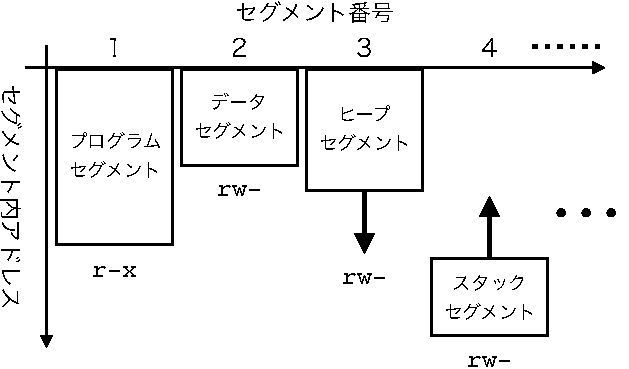
\includegraphics[scale=0.88]{Fig/segment-crop.pdf}
\end{myfig}

\figref{segment}は以下のことを表している.
プログラム,データ,ヒープ,スタックの領域を番号付けされたセグメントにした.
セグメントに付記した\|rwx|はセグメントの保護モードを表している.
セグメントの大きさは内容の大きさとぴったり同じサイズにできるので,
内部フラグメントが生じない.
ヒープ領域は実行時に必要に応じて長くすることができる.
スタックが前に向かって伸びる場合は,
前向きに伸びるセグメントが使いやすい.
IA-32\footnote{
  32bitパーソナルコンピュータで広く使われてきた
  インテル社CPUのアーキテクチャのことである.}は,
前に向かって伸びるセグメントもサポートしている\cite{ia32Segmentation}.

各領域を独立したセグメントにすることで,
\emph{仮想アドレス空間内の領域配置の問題から解放された}.

%==========================================================================
\section{セグメント番号}
仮想アドレスにセグメント番号が新たに必要になった.
セグメント番号を供給するためにCPUに変更が必要になる.
以下では,セグメント番号を提供する方法を考える.

\subsection{命令コード}
機械語命令コードを変更し,
セグメント番号を含める方法が考えられる.
各命令がセグメント番号のために大きくなるので,
プログラムサイズが大きくなる.
\begin{center}
  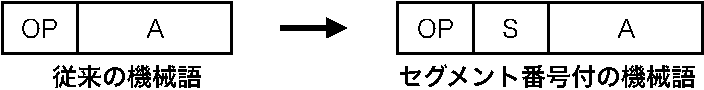
\includegraphics[scale=0.77]{Fig/segmentationInstruction-crop.pdf}
\end{center}

\subsection{カレントセグメントレジスタ}
CPU内部に現在のセグメント番号を格納するレジスタを置く方式である.
別のセグメントへプログラムをジャンプさせる
セグメント間ジャンプ命令(JMPSと仮に命名する),
セグメント間コール命令(CALLSと仮に命名する),
セグメント間リターン命令(RETSと仮に命名する)が
カレントセグメントレジスタに新しいセグメント番号をロードする.

\figref{segmentCall}に模式図を示す.
まず,セグメント1のプログラムが実行される.
この時点ではカレントセグメントはセグメント1なので,
\texttt{LD G0,A}はセグメント1内のデータ\texttt{A}を参照する.

\texttt{CALLS 3:0}はセグメント3の0番地に配置されたサブルーチンを呼び出す.
その際,カレントセグメントレジスタの値と
プログラムカウンタの値がスタックに保存される.
その後,カレントセグメントはセグメント3に,
プログラムカウンタは0に変更される.
サブルーチン実行中のカレントセグメントはセグメント3なので,
サブルーチン中の\texttt{ADD G0,A}はセグメント3のデータ\texttt{A}を参照する.

\texttt{RETS}が実行されるとカレントセグメントレジスタと
プログラムカウンタの値がスタックから復元され,
セグメント1のプログラムの実行が再開される.

\begin{myfig}{btp}{セグメント間のサブルーチンコール}{segmentCall}
  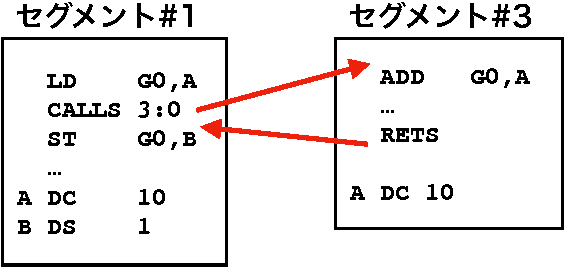
\includegraphics[scale=0.66]{Fig/segmentCall-crop.pdf}
\end{myfig}

IA-32は,プログラム用(CS),データ用(DS),スタック用(SS)等,
数個のカレントセグメントレジスタを持つ.
機械語命令のフェッチにはCS,
データのアクセスにはDS,
スタックの操作にはSSが暗黙の内に使用される\cite{ia32SegmentReg}.

%==========================================================================
\section{セグメンテーション機構}
セグメンテーション機構の模式図を\figref{segmentation}に示す.
CPUが出力したセグメント番号(S)とセグメント内アドレス(A)の組を,
セグメントテーブルを使用して物理アドレスに変換する.

\begin{myfig}{btp}{セグメンテーション機構}{segmentation}
  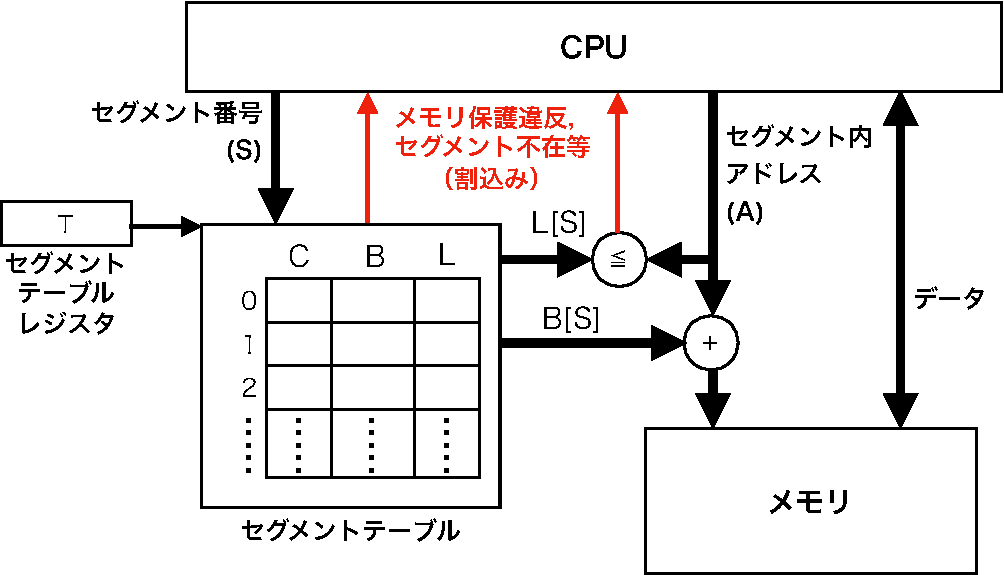
\includegraphics[scale=0.66]{Fig/segmentation-crop.pdf}
\end{myfig}

\subsection{セグメントテーブル}
現在のプロセスが使用できるセグメントの一覧表である.
表の一行(エントリ)が一つのセグメントを表現する.
B(Base)フィールドはセグメントの物理アドレス,
L(Limit)フィールドはセグメントサイズであり,
セグメントテーブルのエントリはリロケーションレジスタと同様な内容を含んでいる.

C(制御)フィールドは,
\tabref{segmentTableAttr}のビットを含んでいる.
V(Valid)ビットが0の場合,そのセグメントはメモリ上に存在しない.
存在しないセグメントをアクセスしようとすると
\emph{セグメント不在割込み}が発生する.
D(Dirty)ビットはセグメントの内容がメモリにロードされた後に
変更されたことを記録する.
メモリが不足してセグメントをスワップアウトする際,
Dビットが0ならセグメントを二次記憶装置へ書き戻す必要がない.
RWX(Read/Write/eXecute)の三ビットはセグメントに対して行って良い操作を表す.
CPUが許可されていない操作を行うとメモリ保護違反割込みが発生する.

\begin{mytable}{btp}{セグメントテーブルCフィールドの例}{segmentTableAttr}
  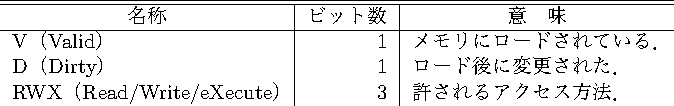
\includegraphics[scale=1.0]{Tbl/segmentTableAttr.pdf}
\end{mytable}

\figref{segmentation}では,
セグメントテーブルが専用のハードウェアとして描かれているが,
セグメントテーブルはメモリ上に置かれる.
セグメントテーブルのアドレスは\emph{セグメントテーブルレジスタ}が
記憶している.
プロセスを切り換える際は,
そのプロセスのセグメントテーブルを指すように
セグメントテーブルレジスタを書き換える.

\subsection{物理アドレスへの変換}
CPUが出力したセグメント番号(S)とセグメント内アドレス(A)の組は,
以下の手順で物理アドレスに変換される.

\begin{enumerate}
\item \emph{セグメントテーブルのエントリ読み出し}\\
  セグメントテーブルは,
  セグメントテーブルレジスタによって示されるメモリ上のアドレスに配置されている.
  セグメント番号をセグメントテーブルのインデクスとして使用し,
  セグメントテーブルの一つのエントリをメモリから読み出す.

\item \emph{Cフィールドのチェック}\\
  読み出したエントリのCフィールドを調べ,
  セグメントがメモリにロードされていない場合や,
  許可されていない種類(RWX)のアクセスをCPUが行おうとしている場合は,
  割込みを発生する.

\item \emph{セグメント内アドレスのチェック}\\
  読み出したエントリのLフィールド(L[S])と
  CPUが出力したセグメント内アドレス(A)を比較する.
  L[S]はセグメントのサイズを表すので,
  AがL[S]以上の場合はセグメント内アドレスがセグメントの後端を越えている.
  メモリアクセスを阻止した上で割込みを発生する.

\item \emph{物理アドレスの計算}\\
  読み出したエントリのBフィールド(B[S])と
  CPUが出力したセグメント内アドレス(A)の和を求める.
  和が物理アドレスである.
\end{enumerate}

\subsection{セグメントテーブルエントリのキャッシング}
前記の物理アドレスへの変換手順では,
メモリアクセスの度にセグメントテーブルを参照していた.
セグメントテーブルの参照はメモリアクセスなので,
メモリアクセス回数が二倍になる.
他のCPUやI/O装置もメモリを使用するので,
メモリへのアクセスは混み合っている.
メモリアクセス回数は少なくすべきである.

一方で,同時に使用されるセグメントの数は多くないので,
必要なテーブルエントリをCPUやMMUにキャッシュすることは容易である.
例えばIA-32では,
カレントセグメントレジスタ(CS,DS,SS等)毎に,
セグメントテーブルエントリのコピーを
裏レジスタ\cite{ia32SegmentHiddenReg}に持つ.
カレントセグメントレジスタの値が変更された時,
自動的に裏レジスタにエントリがコピーされる.
\figref{segmentIa32}にセグメントレジスタと裏レジスタの関係を示す.
セグメントレジスタに格納されるセレクタはセグメント番号に相当する.
裏レジスタはハードウェアが自動的に使用しプログラムからは見えない.

\begin{myfig}{btp}{IA-32のセグメントレジスタと裏レジスタ}{segmentIa32}
  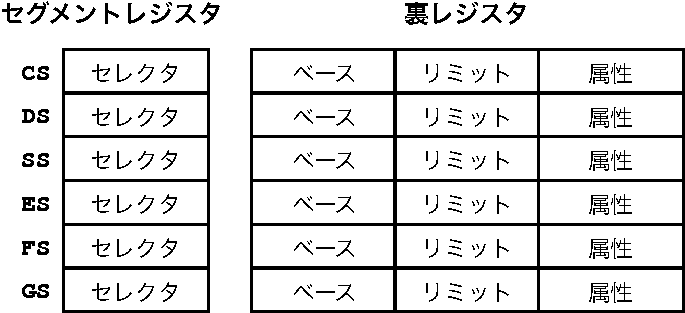
\includegraphics[scale=0.8]{Fig/segmentIa32-crop.pdf}
\end{myfig}

%==========================================================================
\section{セグメンテーション機構による仮想記憶}
プログラム実行中に必要なセグメントだけをメモリにロードするようにする.
これにより,全体がメモリに収まらない大きなプログラムも実行できる.
メモリより大きなプログラムが実行できる点で,
メモリが仮想化されたと言うことができる.
仮想化されたメモリのことを\emph{仮想記憶}と呼ぶ.

\subsection{スワップイン}
セグメントテーブルのVビットが0のセグメントを参照すると,
\emph{セグメント不在割込み}が発生する.
プロセスがセグメント不在割込みを発生すると
オペレーティングシステムに制御が移る.

オペレーティングシステムは,
まず,割込みの原因になったセグメントを
二次記憶装置から読み込む(\emph{スワップイン}する).
次に,セグメントテーブルを書き換える.
最後に割込みを発生した命令の再実行から再開するように
プロセスをディスパッチする.

\subsection{スワップアウト}
オペレーティングシステムがセグメントをスワップインする際に
メモリが不足するかも知れない.
その場合,オペレーティングシステムは適切なセグメントを選択し
二次記憶に追い出し(\emph{スワップアウト}し),
メモリに空きを作らなければならない.
今後,使用されそうに無いセグメントを選択すると良いが,
どのセグメントが該当するか判断することは難しい問題である.

\figref{segmentSwapping}にセグメントが
スワップアウト/スワップインされる様子を示す.
図は新しくセグメント3が必要になりスワップインする様子を表している.
セグメント3をロードするためにはメモリが不足するので,
まず,使用頻度が低いセグメント1をスワップアウトし,
次に,セグメント3をスワップインする.

\begin{myfig}{btp}{セグメントのスワッピング}{segmentSwapping}
  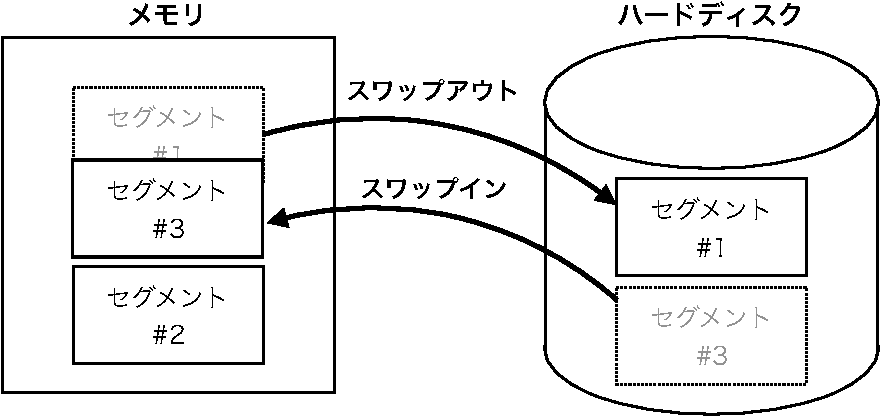
\includegraphics[scale=0.66]{Fig/segmentSwapping-crop.pdf}
\end{myfig}

%==========================================================================
\section{セグメントの共用}
プロセス間でセグメントを共用することでメモリの節約ができる.
プログラムや定数等を格納し,
書き込み禁止のセグメントは複数のプロセスで共用できる.
逆に,書き込みが許可されている
データ,ヒープ,スタックセグメント等は共用できない.
また,セグメントの共用を積極的に利用しプロセス間の共有メモリも実現できる.
\figref{segmentSharing}に三つのプロセスがセグメントを共用している様子を示す.

\begin{myfig}{btp}{セグメントの共用}{segmentSharing}
  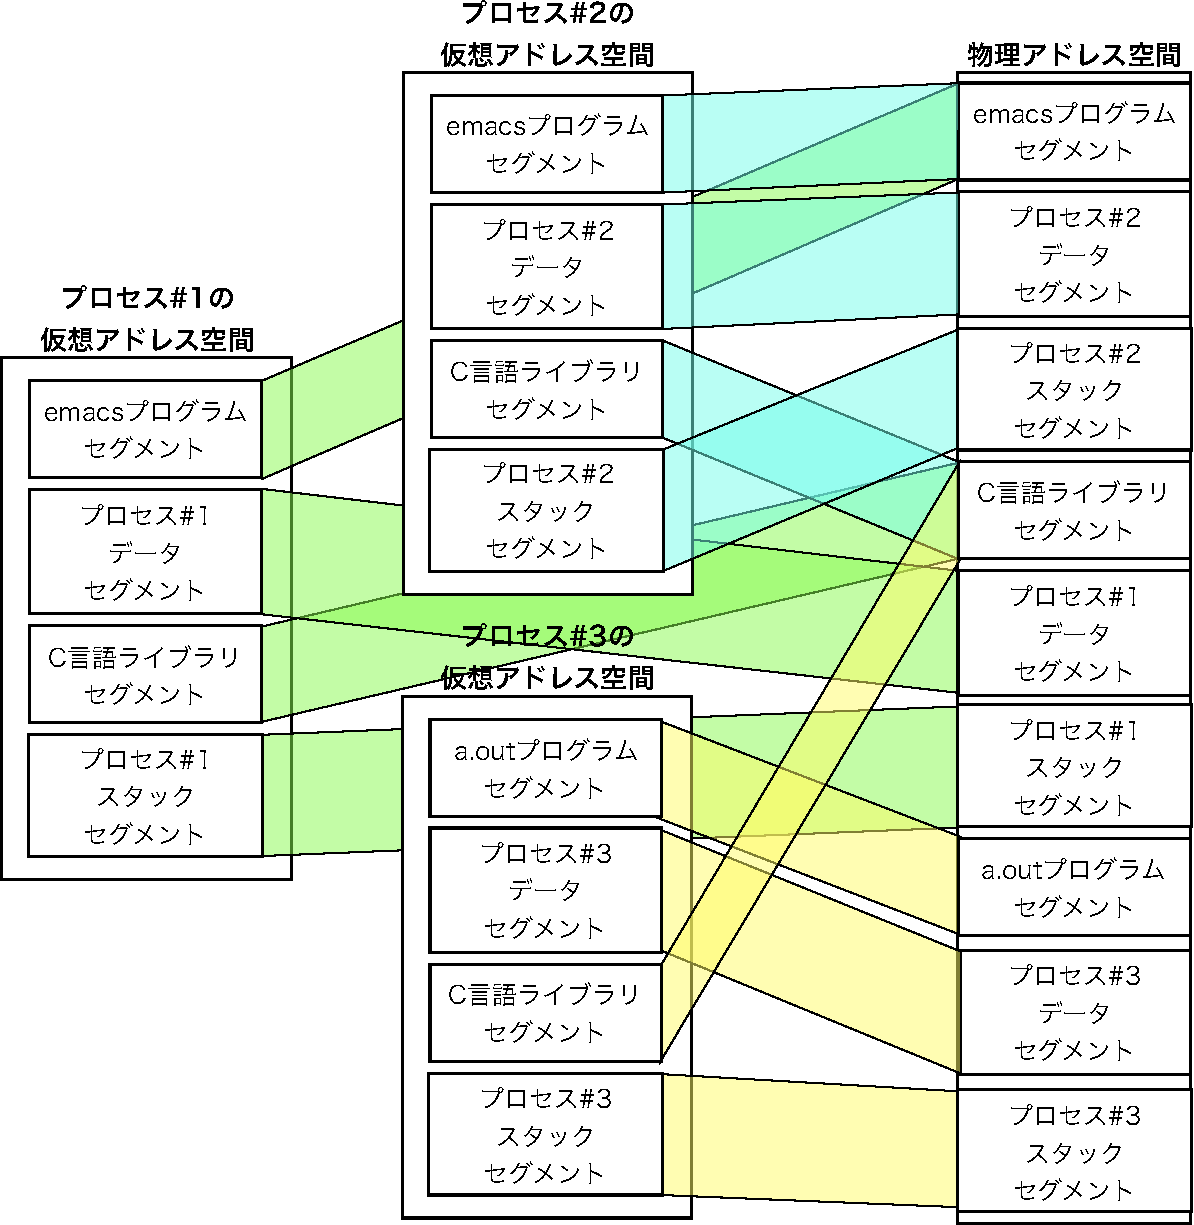
\includegraphics[scale=0.66]{Fig/segmentSharing-crop.pdf}
\end{myfig}

\begin{itemize}
\item C言語ライブラリは,
  C言語で使用する関数(\texttt{printf()}等)を提供する.
  ライブラリはプログラムだけを格納し変更されないので,
  全てのプロセスで共用することができる\footnote{
    本当は,ライブラリが使用するグローバル変数(例えば\texttt{errno})を
    どうするか問題である.
  }.

\item プロセス1とプロセス2はどちらも emacs を実行している.
  プログラムは変更されないので,
  プロセス1とプロセス2で「emacsプログラムセグメント」を共用できる.

\item プロセス3は a.out を実行している.
  プログラムは変更されないが,
  同じプログラムを実行中のプロセスが存在しないので
  「a.out プログラムセグメント」は共用できない.

\item プロセスが書き換えるデータセグメントやスタックセグメントは,
  プロセス毎に内容が異なるので共用できない.
  別々のデータセグメントやスタックセグメントが必要になる.
  プロセス1とプロセス2はどちらも emacs を実行しているが,
  編集している文書が異なるのでデータセグメントの内容も異なるハズである.
\end{itemize}

%==========================================================================
\section{セグメンテーションの利点・欠点}
セグメンテーションの利点と欠点を以下にまとめる.

\subsection*{利点}
\begin{itemize}
\item セグメントには,例えば「C言語ライブラリセグメント」のような,
  論理的な意味を持たせることができる.
\item セグメントの論理的な意味を反映したメモリ保護が可能である.
\item プログラムやデータの共用が容易である.
\item セグメントの長さは自由に決められるので内部フラグメントが発生しない.
\item セグメントの長さは動的に変化させることも可能である.
\item セグメント単位のスワッピングを用いて仮想記憶を実現できる.
\end{itemize}

\subsection*{欠点}
\begin{itemize}
\item 物理アドレス空間に外部フラグメントが生じる.
\item 外部フラグメントの解消にはメモリコンパクションが必要である.
\item 物理メモリ上に連続した領域が必要である.
\item 物理メモリより大きいセグメントを作ることができない.
\end{itemize}

外部フラグメント問題と,
物理メモリサイズによるセグメントサイズの制約を解決するために,
次の章で紹介するページングと組合せてセグメンテーションを利用する
システムもある.
例えば,IA-32はそうである.
IA-32ではセグメンテーション機構が出力する一次元のアドレスを
ページング機構が物理アドレスに変換する.

%==========================================================================
\section{まとめ}
本章では,領域の性格に合わせたメモリ保護ができる
高度な管理機構であるセグメンテーションを紹介した.
セグメントには論理的な意味付けをすることができる.
論理的な意味付けに合わせてメモリ保護モードを設定したり,
プログラム間で共有したりする.
また,セグメントは可変長なので内部フラグメントを生じない.
しかし,外部フラグメントを生じるのでメモリコンパクションを必要とする.

セグメントのスワッピングによる仮想記憶を実現できるが,
物理メモリより大きなセグメントを作ることはできない.
そこで,ページングとセグメンテーションを組み合わせて利用するシステムがある.

%==========================================================================
\section*{練習問題}
\begin{enumerate}
  \renewcommand{\labelenumi}{\ttfamily\arabic{chapter}.\arabic{enumi}}
  \setlength{\leftskip}{1em}
\item セグメントテーブルが次のような状態の時,以下の問に答えなさい.
  なお,仮想アドレスは「セグメント番号:物理アドレス」と表記する.
  また,物理アドレスは8ビットとする.
  \begin{center}
    \begin{tabular}{r |r|r|r|}
      \multicolumn{1}{c}{} &
      \multicolumn{1}{c}{C} &
      \multicolumn{1}{c}{B} &
      \multicolumn{1}{c}{L} \\
      \cline{2-4}
      0   & V=1 & 0x30 & 0x20 \\
      1   & V=1 & 0x80 & 0x30 \\
      2   & V=1 & 0x00 & 0x20 \\
      3   & V=0 & 0x50 & 0x20 \\
      ... & ... & ... & ... \\
      \cline{2-4}
    \end{tabular}
  \end{center}
  \begin{enumerate}
  \item 次の仮想アドレスに対応する物理アドレスを答えなさい.
    但し,物理アドレスに変換できない場合はエラーと答えなさい.
    \begin{enumerate}
    \item \texttt{0x0:0x10}
    \item \texttt{0x1:0x10}
    \item \texttt{0x1:0x40}
    \item \texttt{0x2:0x10}
    \item \texttt{0x2:0x20}
    \item \texttt{0x3:0x10}
    \end{enumerate}
  \item セグメントの配置を記入した
    物理アドレス空間のメモリマップを作成しなさい.
  \end{enumerate}
  \item スタックセグメントを意識した
    \emph{前向きに伸びるセグメント}も利用可能な
    セグメンテーション機構を設計しなさい.
    \begin{enumerate}
    \item セグメントテーブルに必要な変更は?
    \item \figref{segmentation}に必要な変更は?
    \item 他に必要な変更は?
    \end{enumerate}
\end{enumerate}
